\documentclass[12pt,addpoints,a4paper]{exam}
\usepackage{tikz}
\begin{document}
\begin{center}
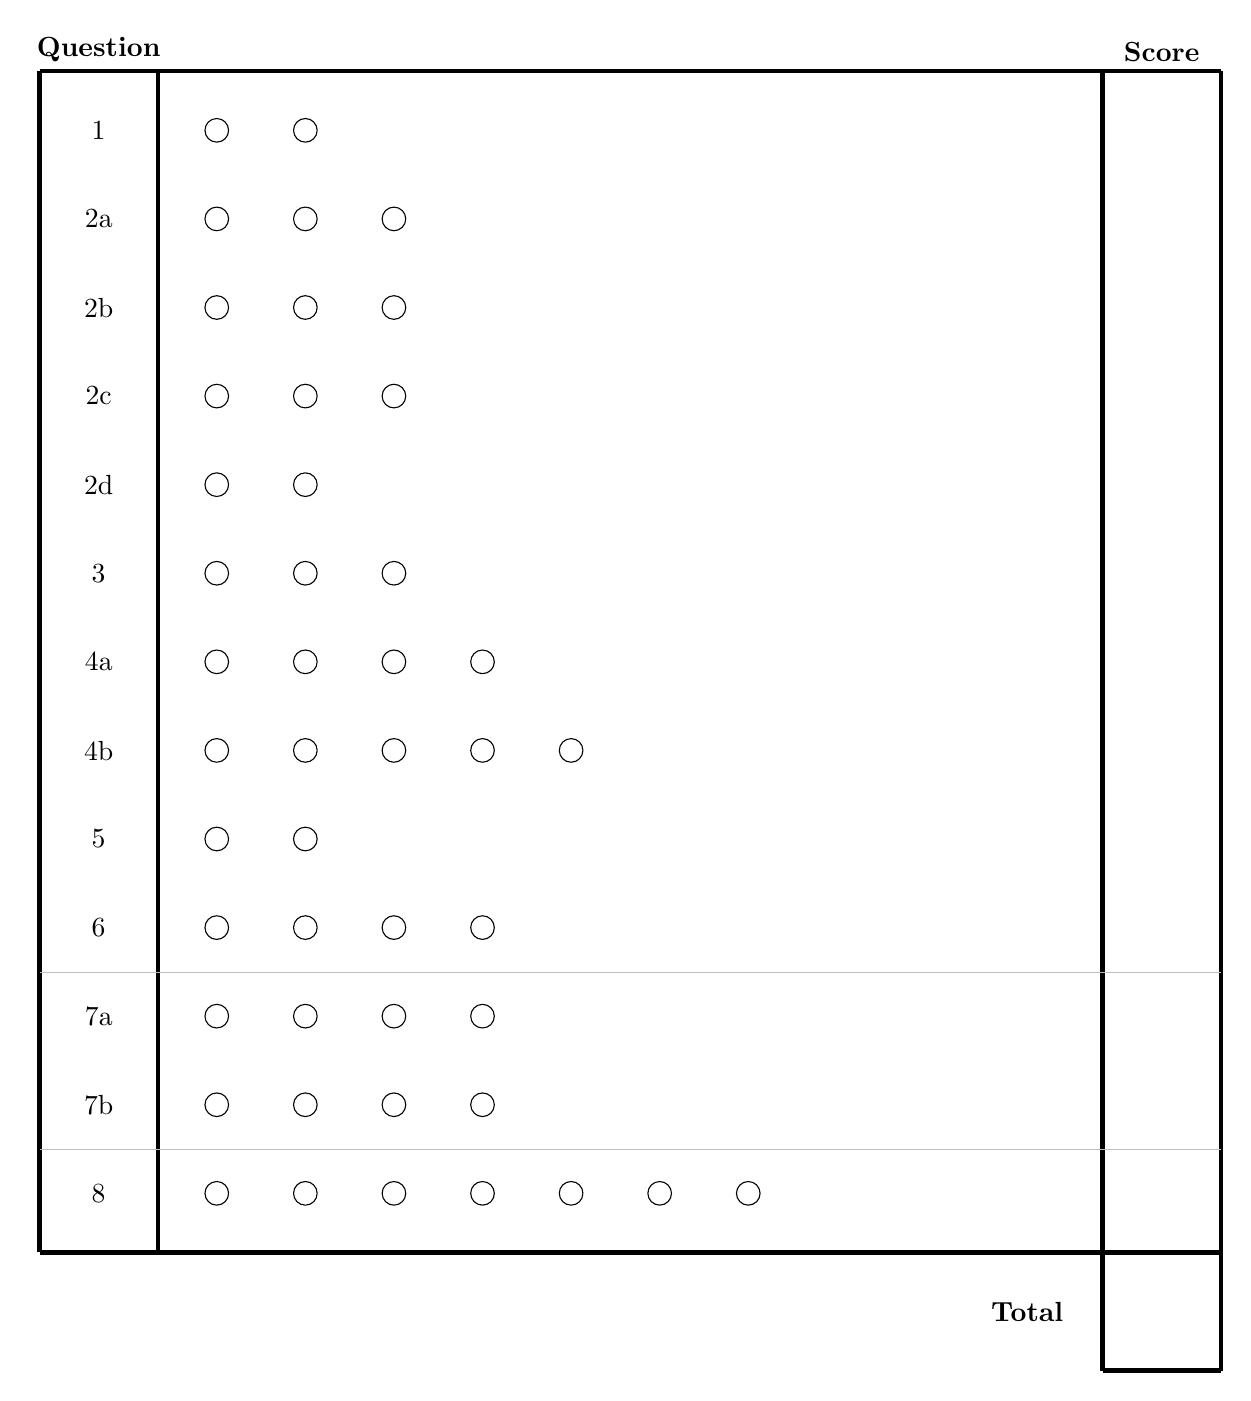
\begin{tikzpicture}[scale=.75]
\draw[ultra thick] (-10,-1.5)--(10,-1.5);
\draw[ultra thick] (-10,-1.5)--(-10,-21.5);
\draw[ultra thick] (-8,-1.5)--(-8,-21.5);
\draw[ultra thick] (8,-1.5)--(8,-23.5);
\draw[ultra thick] (10,-1.5)--(10,-23.5);
\draw[ultra thick] (-10,-21.5)--(10,-21.5);
\draw[ultra thick] (8,-23.5)--(10,-23.5);
\draw (7.5,-22.5) node[left]{\textbf{Total}};
\draw (9,-1.5) node[above]{\textbf{Score}};
\draw (-9,-1.5) node[above]{\textbf{Question}};
\draw (-9,-2.5) node{$1$};
\foreach \x in {0,1.5}
\draw (-7+\x,-2.5) circle (0.2cm);
\draw (-9,-4) node{$2\mathrm{a}$};
\foreach \x in {0,1.5,3}
\draw (-7+\x,-4) circle (0.2cm);
\draw (-9,-5.5) node{$2\mathrm{b}$};
\foreach \x in {0,1.5,3}
\draw (-7+\x,-5.5) circle (0.2cm);
\draw (-9,-7) node{$2\mathrm{c}$};
\foreach \x in {0,1.5,3}
\draw (-7+\x,-7) circle (0.2cm);
\draw (-9,-8.5) node{$2\mathrm{d}$};
\foreach \x in {0,1.5}
\draw (-7+\x,-8.5) circle (0.2cm);
\draw (-9,-10) node{$3$};
\foreach \x in {0,1.5,3}
\draw (-7+\x,-10) circle (0.2cm);  
\draw (-9,-11.5) node{$4\mathrm{a}$};
\foreach \x in {0,1.5,...,4.5}
\draw (-7+\x,-11.5) circle (0.2cm);
\draw (-9,-13) node{$4\mathrm{b}$};
\foreach \x in {0,1.5,...,6}
\draw (-7+\x,-13) circle (0.2cm);
\draw (-9,-14.5) node{$5$};
\foreach \x in {0,1.5}
\draw (-7+\x,-14.5) circle (0.2cm);
\draw (-9,-16) node{$6$};
\foreach \x in {0,1.5,...,4.5}
\draw (-7+\x,-16) circle (0.2cm);
\draw[very thin, gray!50] (-10,-16.75)--(10,-16.75);
\draw (-9,-17.5) node{$7\mathrm{a}$};
\foreach \x in {0,1.5,...,4.5}
\draw (-7+\x,-17.5) circle (0.2cm);
\draw (-9,-19) node{$7\mathrm{b}$};
\foreach \x in {0,1.5,...,4.5}
\draw (-7+\x,-19) circle (0.2cm);
\draw[very thin, gray!50] (-10,-19.75)--(10,-19.75);
\draw (-9,-20.5) node{$8$};
\foreach \x in {0,1.5,...,9}
\draw (-7+\x,-20.5) circle (0.2cm);
\end{tikzpicture}
\end{center}
\end{document}